\documentclass[a4paper,12pt]{article}

\usepackage{url}
\usepackage{epsfig}
\usepackage{graphics}
\usepackage{fancyhdr}
\usepackage[parfill]{parskip} % Activate to begin paragraphs with an empty line rather than an indent
\usepackage{amsmath}
\usepackage{natbib}
\usepackage{subfigure}
\usepackage{svg}
\usepackage[T1]{fontenc}
\usepackage[utf8]{inputenc}
\usepackage{amsmath,amssymb}
\usepackage[russian,english]{babel}
\graphicspath{{pictures/}}

% SVG Options
\setsvg{inkscape = inkscape -z -D}
\setsvg{svgpath = pictures/}

\title{Carl Bildt Tweets: A comparison of regular and constrained Markov chains for text generation}
\author{\hspace*{-0.5cm}
Group Ain't intelligent\\
\hspace*{-1cm}\begin{tabular}{cccc}
Viktor Bj\"{o}rkholm & Jesper Br\"{a}nn & Daniel Duberg & Jakob Tidestr\"{o}m\\
92-11-17 & 92-09-30 & 93-01-17 & 90-10-04 \\
viktorbj@kth.se & jbrann@kth.se & dduberg@kth.se & jakobti@kth.se \\
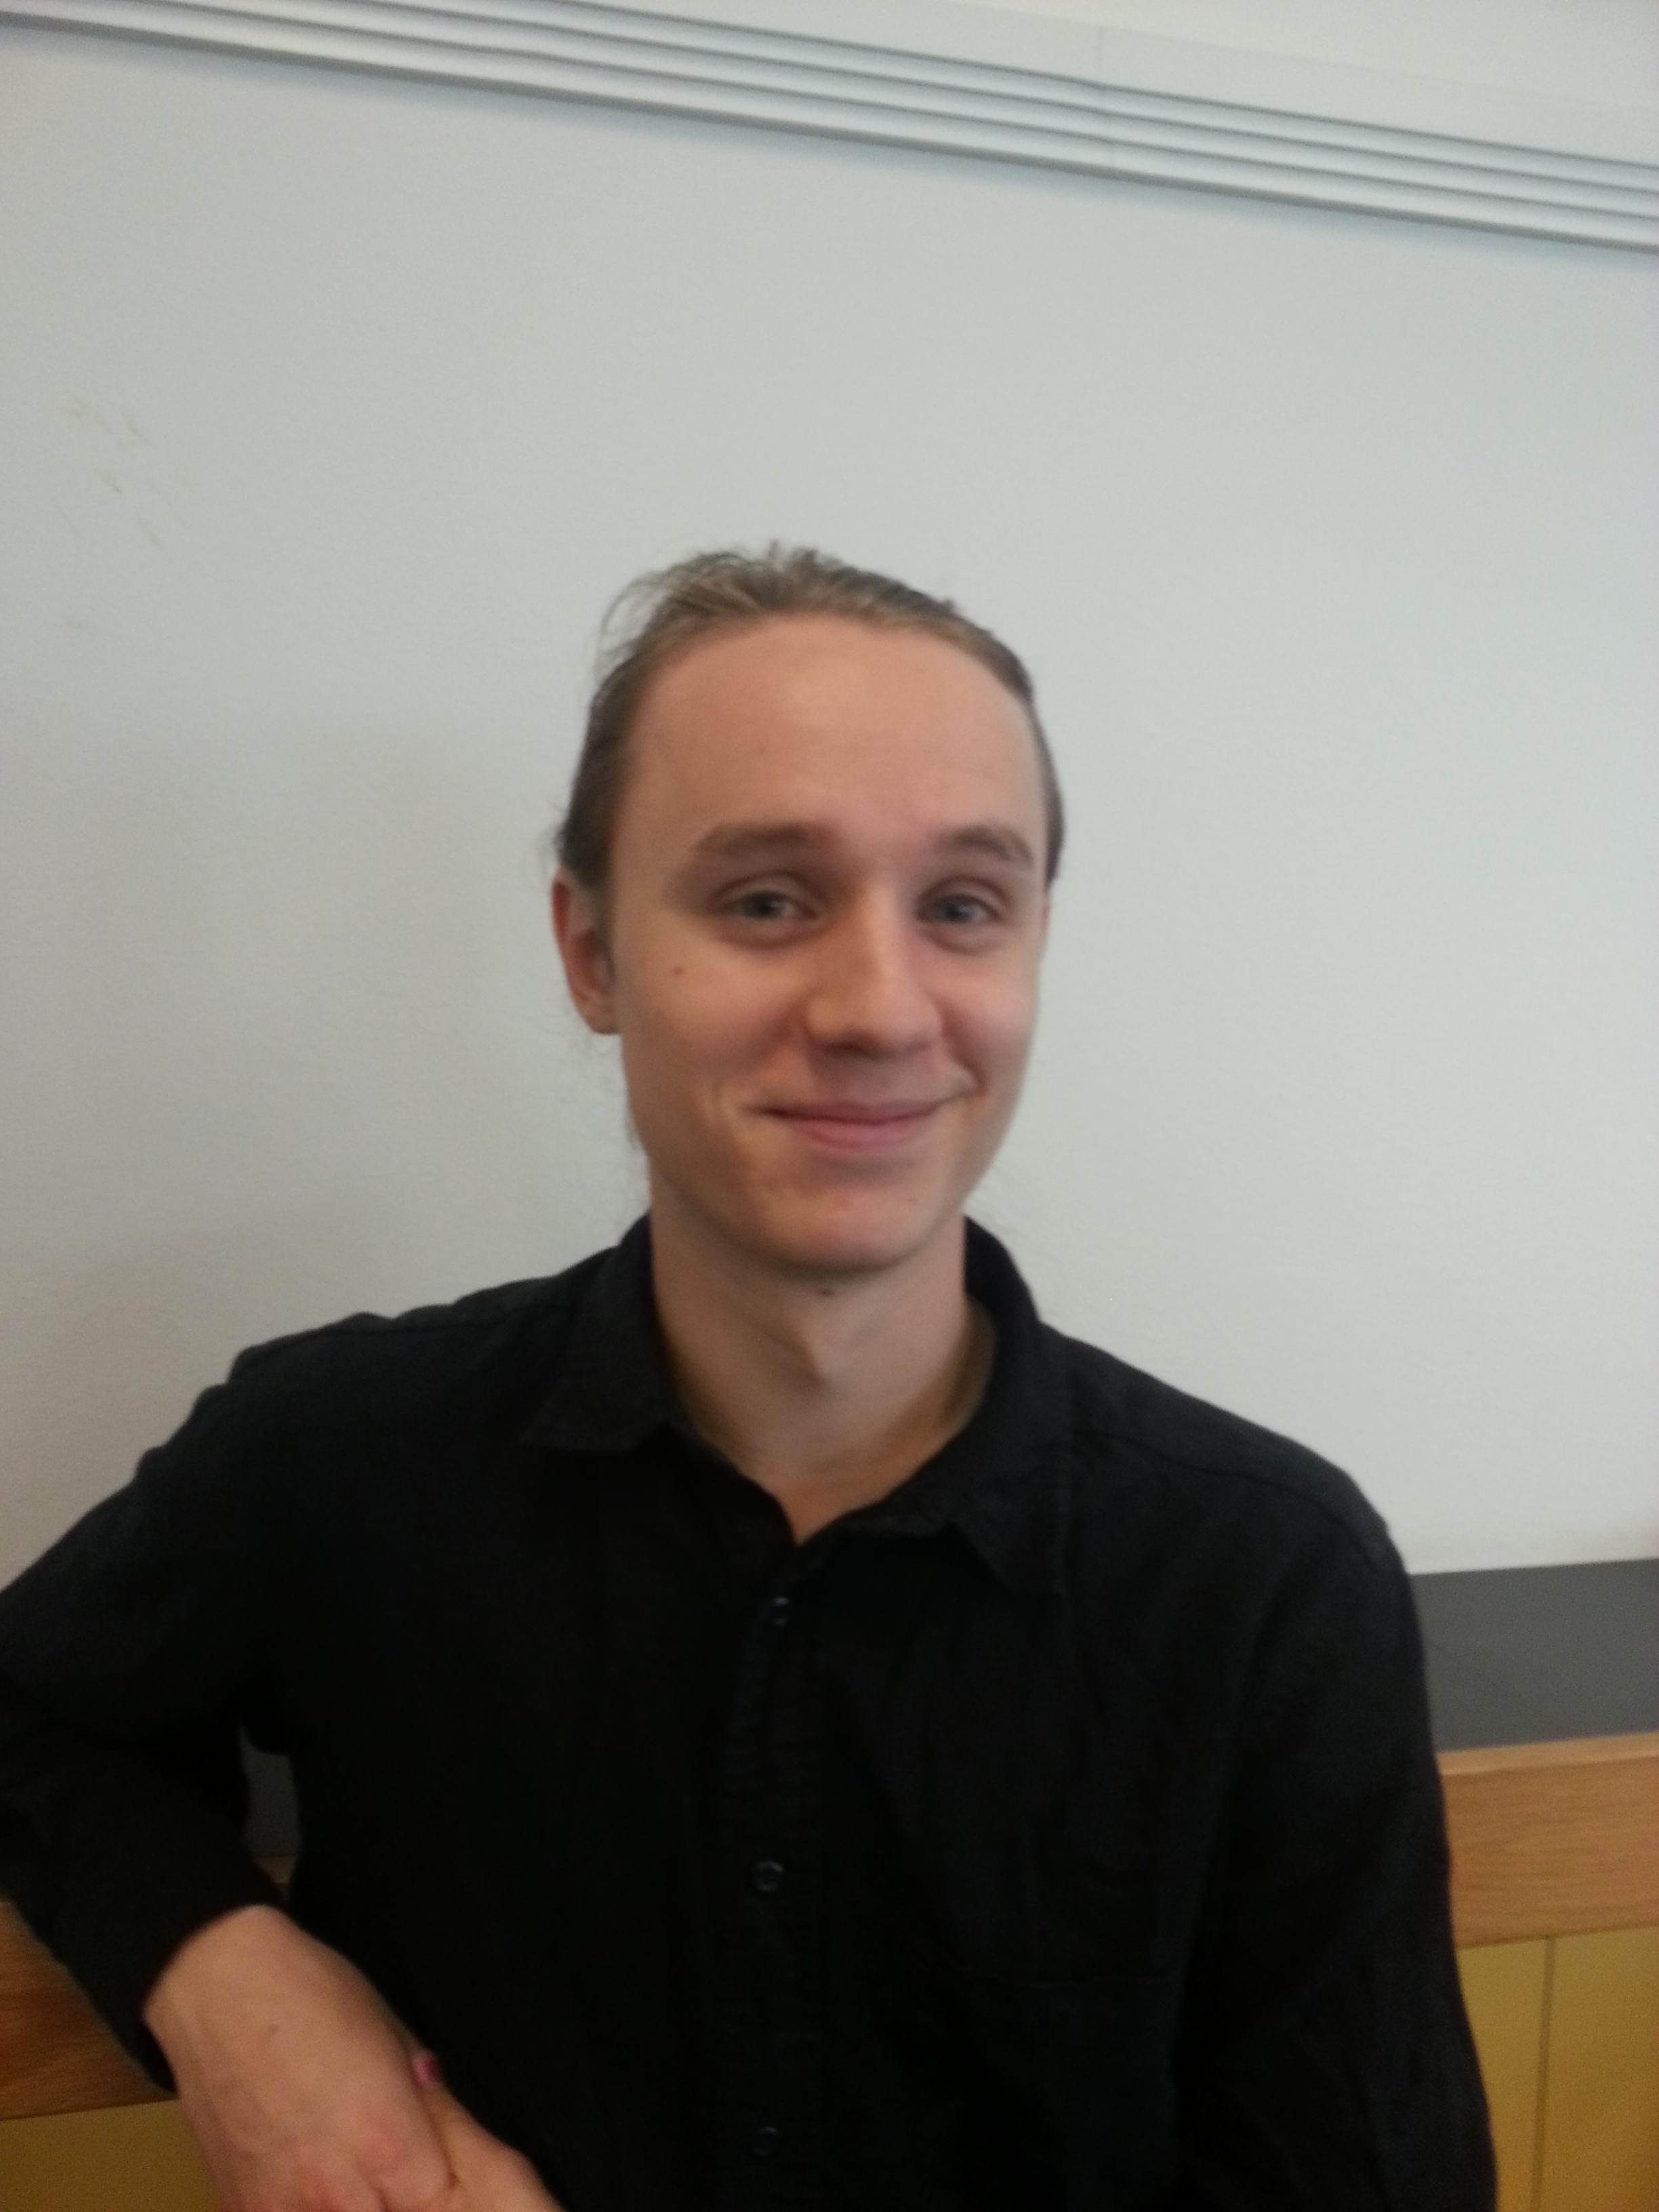
\includegraphics[width=0.13\linewidth, trim=125 125 125 125, clip=true]{viktorbjorkholm} & 

\includegraphics[width=0.13\linewidth, trim=125 125 125 125, clip=true]{jesperbrann} & 
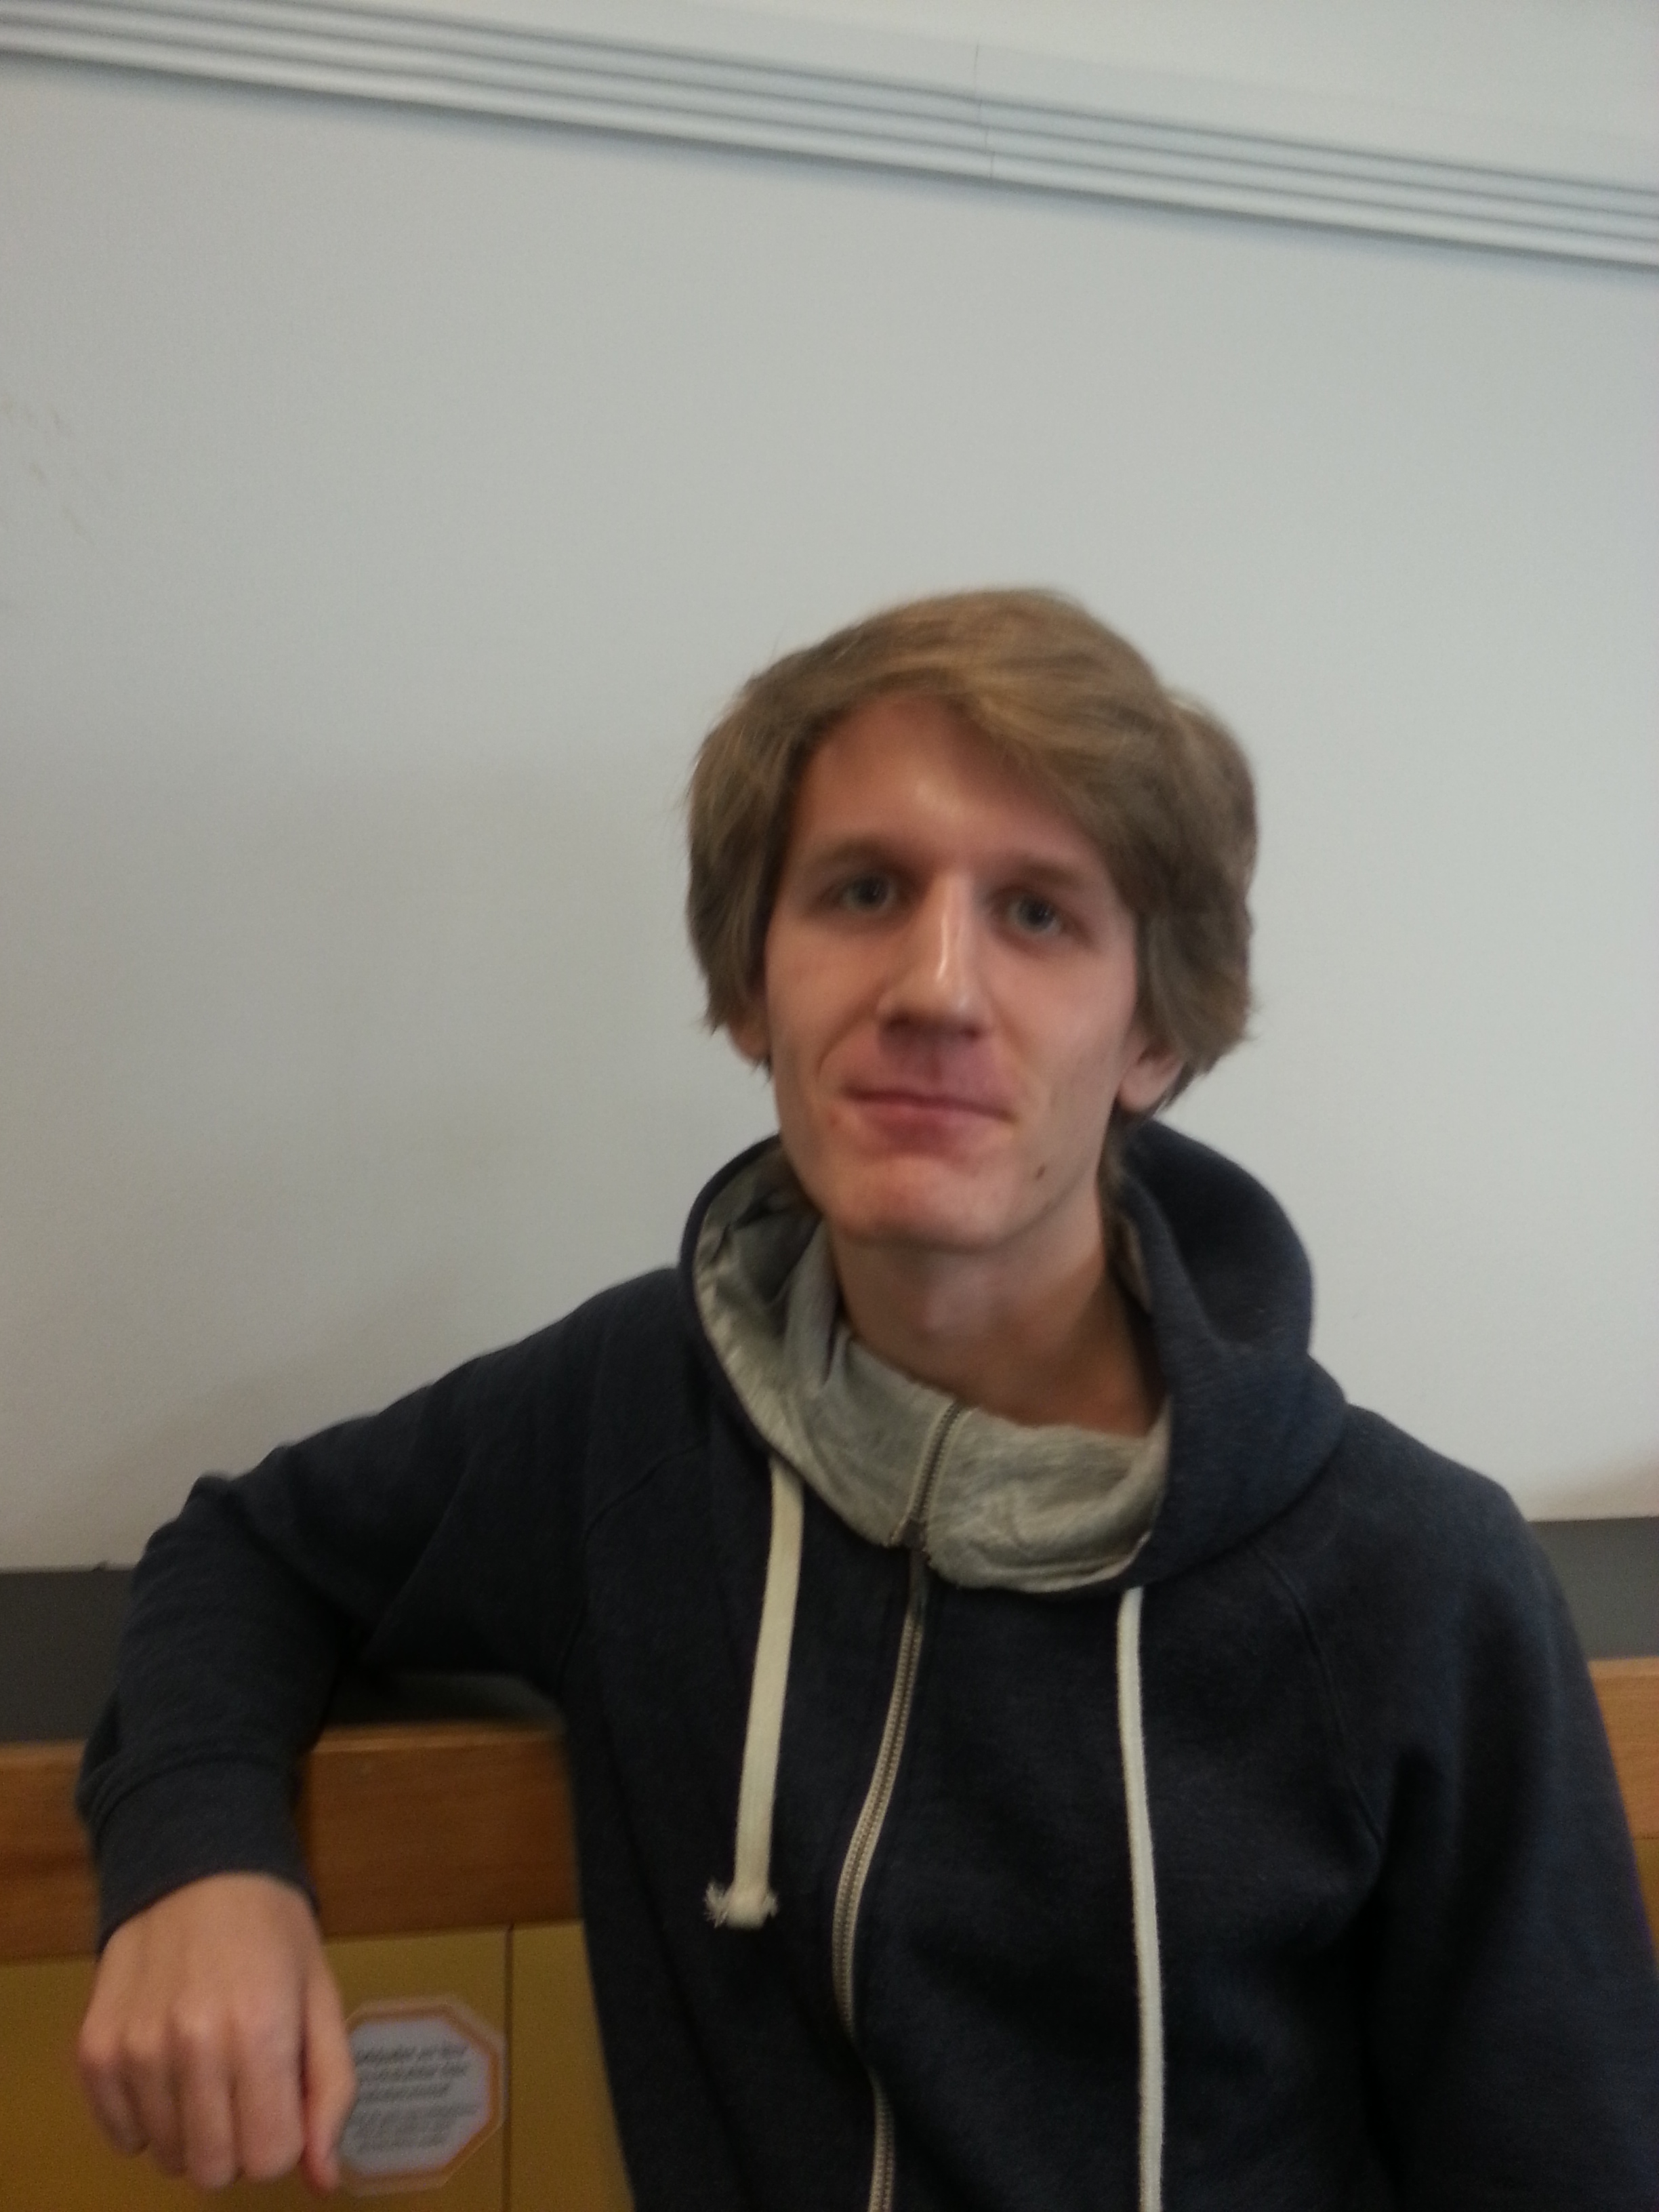
\includegraphics[width=0.13\linewidth, trim=125 125 125 125, clip=true]{danielduberg} & 
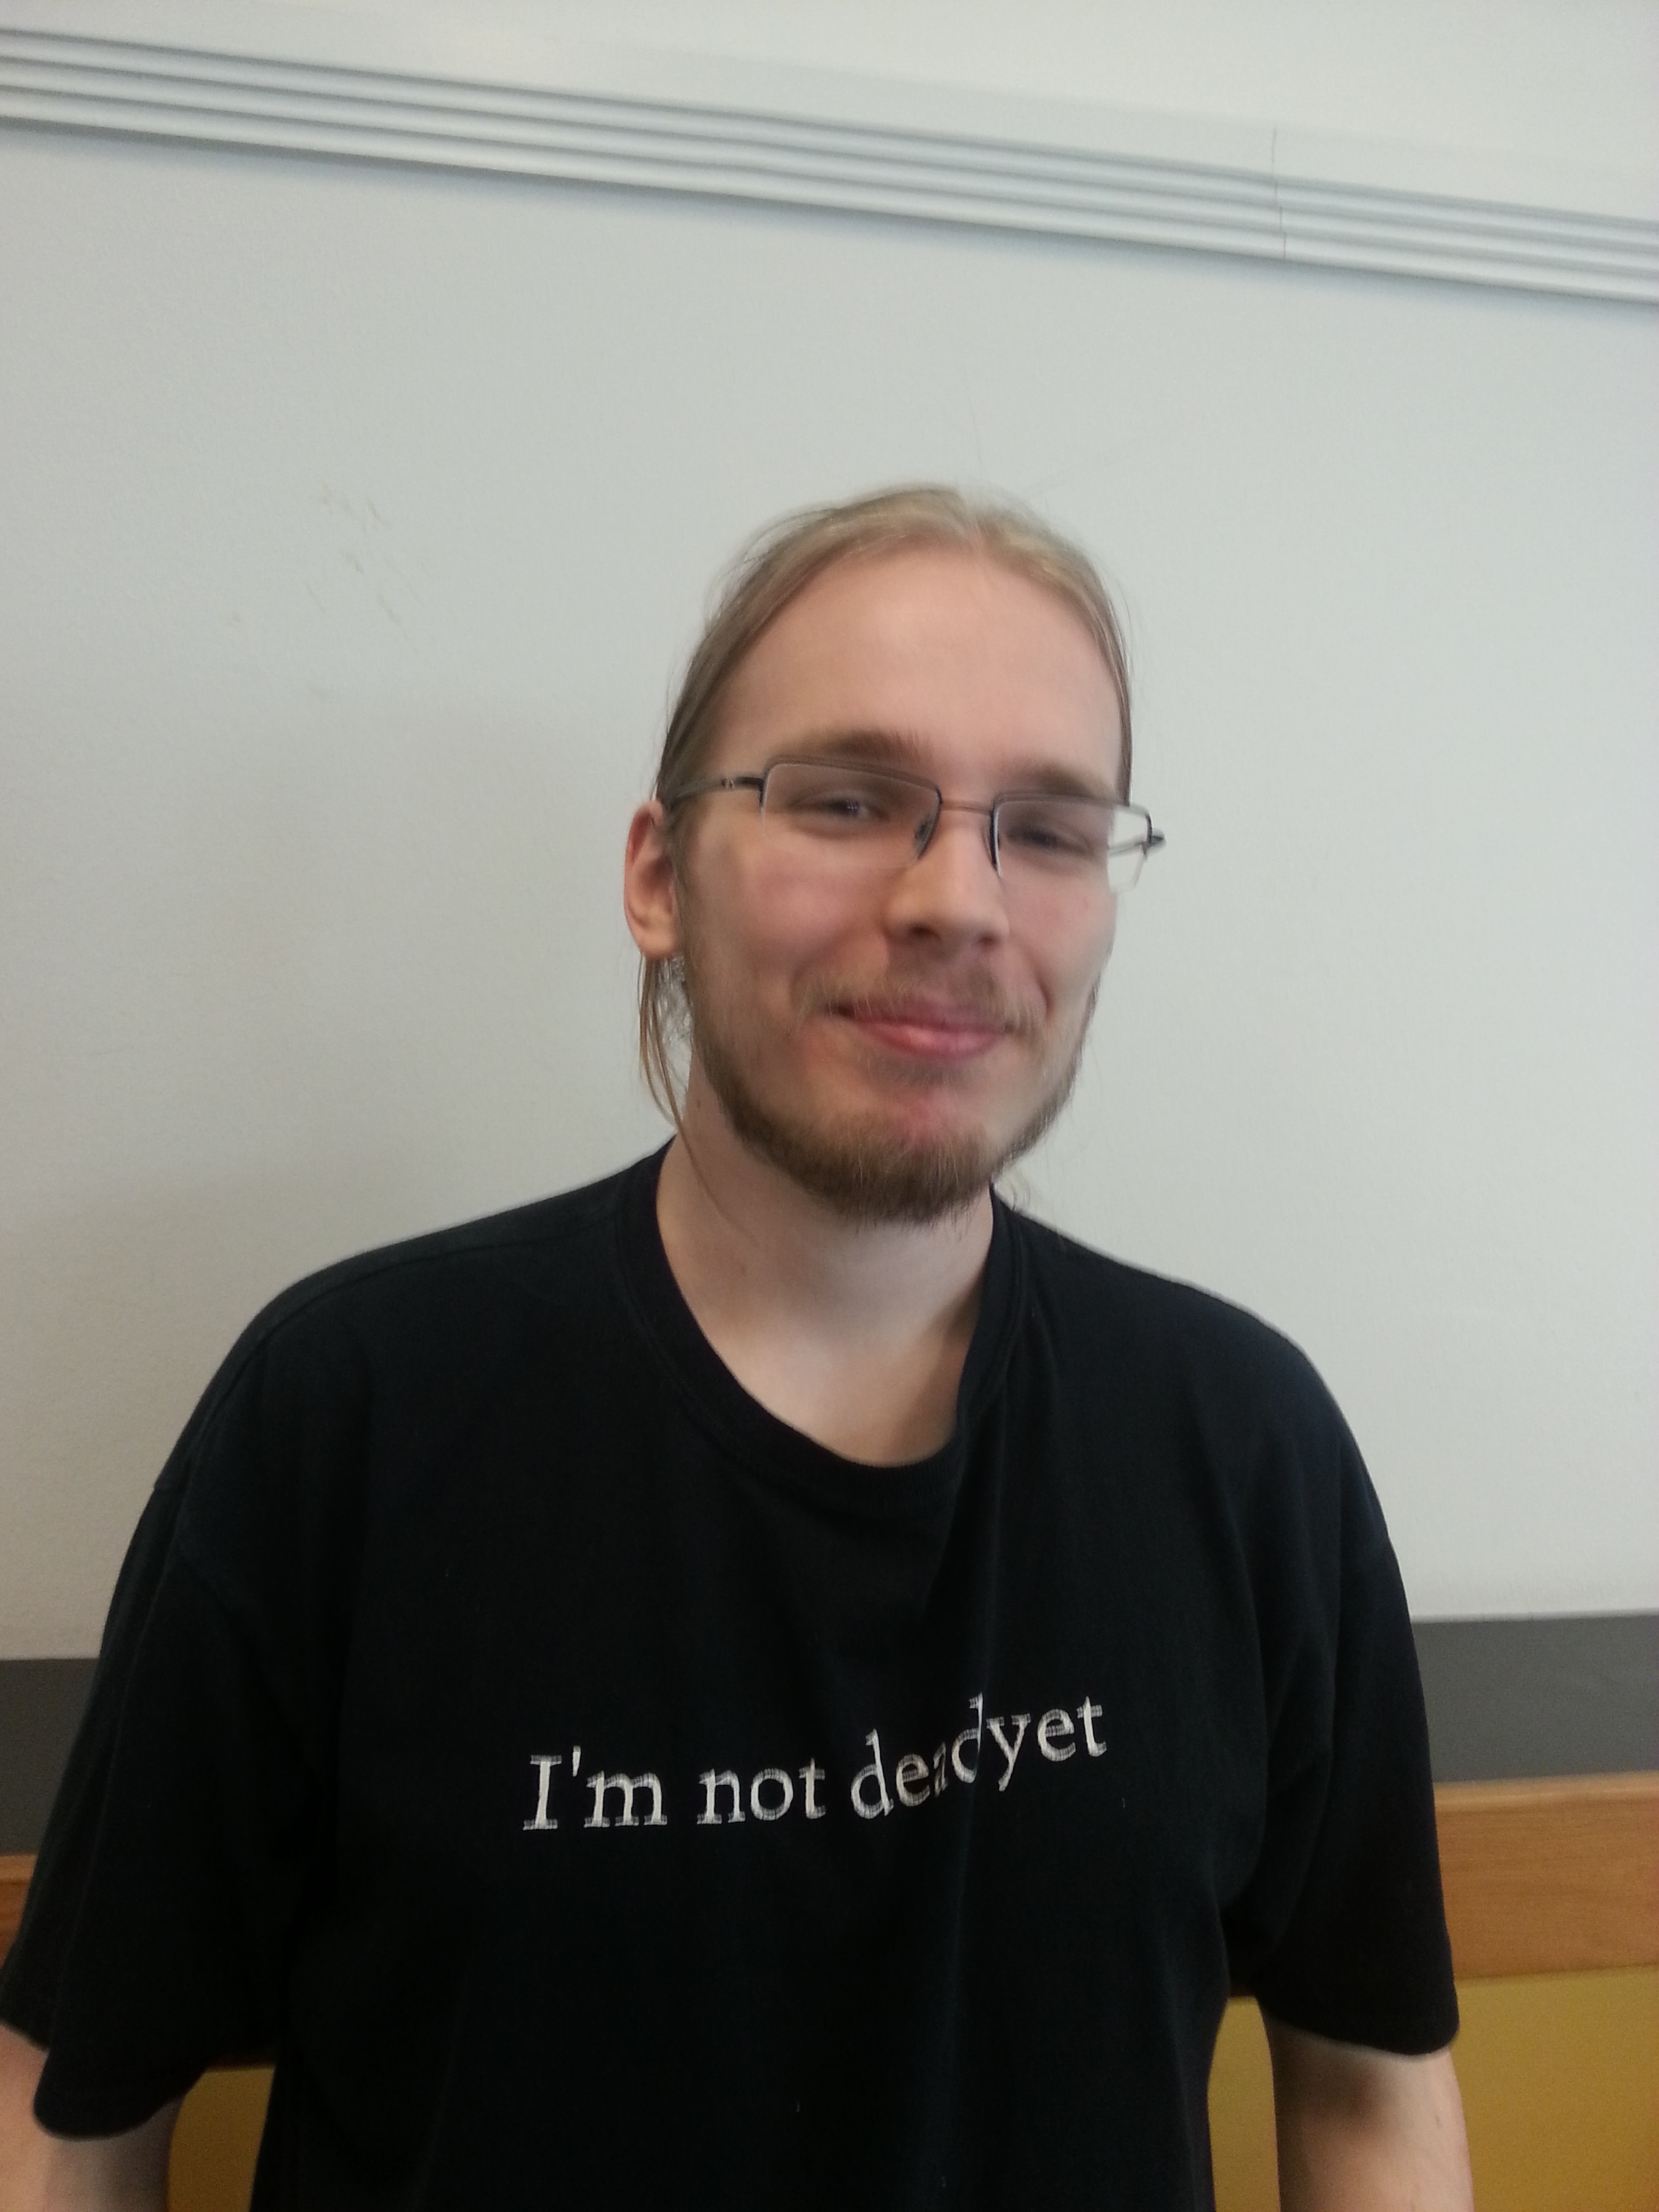
\includegraphics[width=0.13\linewidth, trim=125 125 125 125, clip=true]{jakobtidestrom}
\end{tabular}} 
% Normally there will not be any pictures but we want
% these so that we can connect faces to names in the course
% We also want birthdates so that we can tell people with the same
% name apart
\date{}

\pagestyle{fancy}
\setlength{\headheight}{15pt}
\fancyhf{}
\lhead{DD2380 ai14} % DO NOT REMOVE!!!!
\rhead{V. Bj\"{o}rkholm, J. Br\"{a}nn, D. Duberg, J. Tidestr\"{o}m} %% UPDATE WITH YOUR NAMES

\begin{document}

\maketitle
\thispagestyle{fancy}

\begin{abstract}
This paper explores the difference in result when generating twitter messages that seem to come from a former Swedish foreign minister, Carl Bildt, using two natural language generation based techniques that build on each other.
The outcome of the methods were indeed tweets seeming to originate from Carl Bildt with a subject that circulated around foreign politics. 
The most reliable ones however were mainly copied directly from his feed; this problem is addressed using the methods discussed in this paper. The methods used in this paper are Markov chains with and without constraints to generate tweets, suggestions are also given on improvement of our technique.


\end{abstract}


\clearpage

%%%%%%%%%%%%%%%%%%%%%%%%%%%%%%%%%%%%%%%%%%%%%%%%%%%%%%%%%%%%%
%%%%%%%%%%%%%%%%%%%%%%%%%%%%%%%%%%%%%%%%%%%%%%%%%%%%%%%%%%%%%
\section{Introduction}
\label{sec:intro}

This paper aims to develop an understanding on refining natural language text generation.
Natural Language Generation (NLG) is an area of research within the field of Artificial Intelligence. 
The purpose of NLG is to generate text that is semantically correct in order to make communication with computer systems more natural and understandable for users.

Within this paper the difference in quality of two different approaches to text generation is shown. 
One of these approaches is using Markov chains, also known as n-grams. 
These n-grams take \textit{n} words in sequence and uses a corpus of text to determine what the most probable next word is. 
Using a larger \textit{n} in an n-gram means that more text is copied straight from the corpus, 
however this also means that there is a higher likelihood that the text being generated is meaningful. 

This method is contrasted using constrained Markov chains. 
The main constraint of the Markov chains is that two words following each other will have the same sequence of part-of-speech (POS) as the corpus.
POS is a concept within NLG that divides a text into the different linguistical categories of the words within it.

The aim is to show that using this constraint on the Markov chain, sentences will have a greater diversity but still be as semantically correct as just using a n-gram.
Since the problem with larger n:s within n-grams is that text is copied straight from the corpus, 
the constraint will hopefully help us create semantically correct sentences with a greater diversity from the corpus.

To be able to show differences in these two approaches tweets are generated for a specific person.
This paper builds upon the work by \cite{shannon48} for the theory of implementing an n-gram, a description on generating and parsing corpuses by \citep{Corpus}
and the work by \citealp{McBarb} to implement constraints on the n-gram.
   
\subsection{Contribution}

In order to observe the difference in the result a bi-gram of POS is implemented on to a tri-gram. 
As mentioned above a problem with n-grams with too high \textit{n:s} is that parts of the corpus is copied if said corpus does not contain a large variation of similar sentences, 
so that a given start of \textit{n} words does not automatically lead to one sentence finish. i.e. a larger corpus is needed for larger \textit{n:s}.
To be able to keep a smaller and diverse corpus the bi-gram of POS tags is applied on top of the n-gram to allow the program to select words of a common word type order and with a greater diversity than naturally occurs in the corpus.

This paper's main contribution to the field is that it evaluates putting said bi-gram constraint upon the regular Markov chain and doing it for short message generation.
The research area this paper is based on focus on generating text that fits a theme or rhythm whereas the concept is generalized by creating text that is not constrained by a pre-written sequence of POS. 
The approach is that the model is trained with two types of information, thus the contribution to the field lies in examining how the combination of these two approaches improves the general natural language generation.

\subsection{Outline}
It is explained how \citep{shannon48}, \citep{Corpus} and \cite{McBarb} use NLG in section~\ref{sec:relwork} and also explained how that research has affected this papers. 
In section~\ref{sec:method} the details on how the algorithm works is explained, 
examples are also given to explain in detail what the difference between the two methods that are compared. 
This is complemented with details regarding this paper's specific implementation of the algorithm in section~\ref{sec:impl}. 
The data from running the algorithm is explained, reviewed and evaluated in section~\ref{sec:exps}. Lastly in section~\ref{sec:summary} the results are summarized and it is discussed how the experiments in this paper can be further improved.

%%%%%%%%%%%%%%%%%%%%%%%%%%%%%%%%%%%%%%%%%%%%%%%%%%%%%%%%%%%%%
%%%%%%%%%%%%%%%%%%%%%%%%%%%%%%%%%%%%%%%%%%%%%%%%%%%%%%%%%%%%%
\section{Related work}
\label{sec:relwork}
\cite{shannon48} goes through the first basic steps in how to naively generate text from a corpus with Markov chains. 
He explains in depth how Markov chains can be used to generate real sounding English words from letters and also sentences from words. 
N-grams of different orders are implemented and tried which according to Shannon would generate output more similar to the content of the corpus with the higher orders. 
The difference between the different orders of Markov chains lies in how many preceding states that are taken in consideration.
The Markov chain used in this paper was built up with a transition matrix where the values of the rows in a column represent the probability of moving from the state of the column to the state of the row. The probabilities of the transitions between the different states is taught to the transition matrix by iterating through the corpus. This concept is introduced by Shannon and proven to work in his paper.
His approach was novel at the time however it is a staple in modern text generation. 


In the in-proceedings by \cite{Corpus}, they describe the process of building a corpus for a natural language generation system with different user requests and demands that constrain the corpus. 
The corpus consists of example output that the NLG will imitate and the user requests should be applied through modifying and simplifying the corpus according to them.
Since the corpus should consist of example output, and it is text that should imitate tweets that is going to be generated in this paper, the corpus used is populated with tweets.
We play the role of our own users since we are the ones with demands on the generated text and we need to generate a corpus that is usable by our algorithms. Thus, as \citep{Corpus} describe things from the corpus are removed upon generating it, such as hash-tags and URL:s.


The work on actually constraining the Markov chain is built upon \cite{McBarb} work, 
where the authors generated lyrics from different artists using Markov chains with constraints. 
These were to be generated in a specific style and with a rhythm, to simulate real lyrics from a large span of artists, which is achieved by applying constraints on a tri-gram, a Markov chain of order 2.
They use POS templates to fit the correct poetic metre, these templates are not generated by their algorithm, but rather handcrafted to get a desirable result.
The research from their paper was used to be able to apply constraints upon a tri-gram, or rather a Markov chain in general. Similarily this paper utilize a part-of-speech template of sorts, but diverge a bit from their paper by not handcrafting them and instead letting the algorithm generate them based on the corpus.


%%%%%%%%%%%%%%%%%%%%%%%%%%%%%%%%%%%%%%%%%%%%%%%%%%%%%%%%%%%%%
%%%%%%%%%%%%%%%%%%%%%%%%%%%%%%%%%%%%%%%%%%%%%%%%%%%%%%%%%%%%%
\section{Our method}
\label{sec:method}
Our method that forms the basis of this paper is generating Twitter messages with the use of both Markov chains and constrained Markov chains and to compare the two methods with each other.
The theory is that constraining an Markov chain will yield better and more diverse text being generated. 
In section~\ref{sec:exps} where we explain our experiments and data we use a second order Markov chain, 
for the sake of explanation we assume a first order Markov chain is used to explain how the method works. 
In a limited corpus such as the following: \\

\begin{tabular}{r | l}
``Rolf has a dog.`` & Noun $\to$ verb $\to$ singular quantifier $\to$ noun \\
``Rolf owns a dog.`` & Noun $\to$ verb $\to$ singular quantifier $\to$ noun \\
``Rolf can not walk his dog.`` & Noun $\to$ modal $\to$ adverb $\to$ verb $\to$ pronoun $\to$ noun \\
\end{tabular}

This corpus generates a Markov chain that looks like figure 1a, with the edges being the probabilities for the specific transitions. 
In the figure the specific part-of-speech is included in the states beneath the words from the corpus. 
If we then add constraints from a transition matrix, built up from POS-analysis of the same corpus we are given the new chain that is seen in figure 1b.

\begin{figure}[h!]
  \hfill
  \subfigure[Bi-gram of the limited corpus]{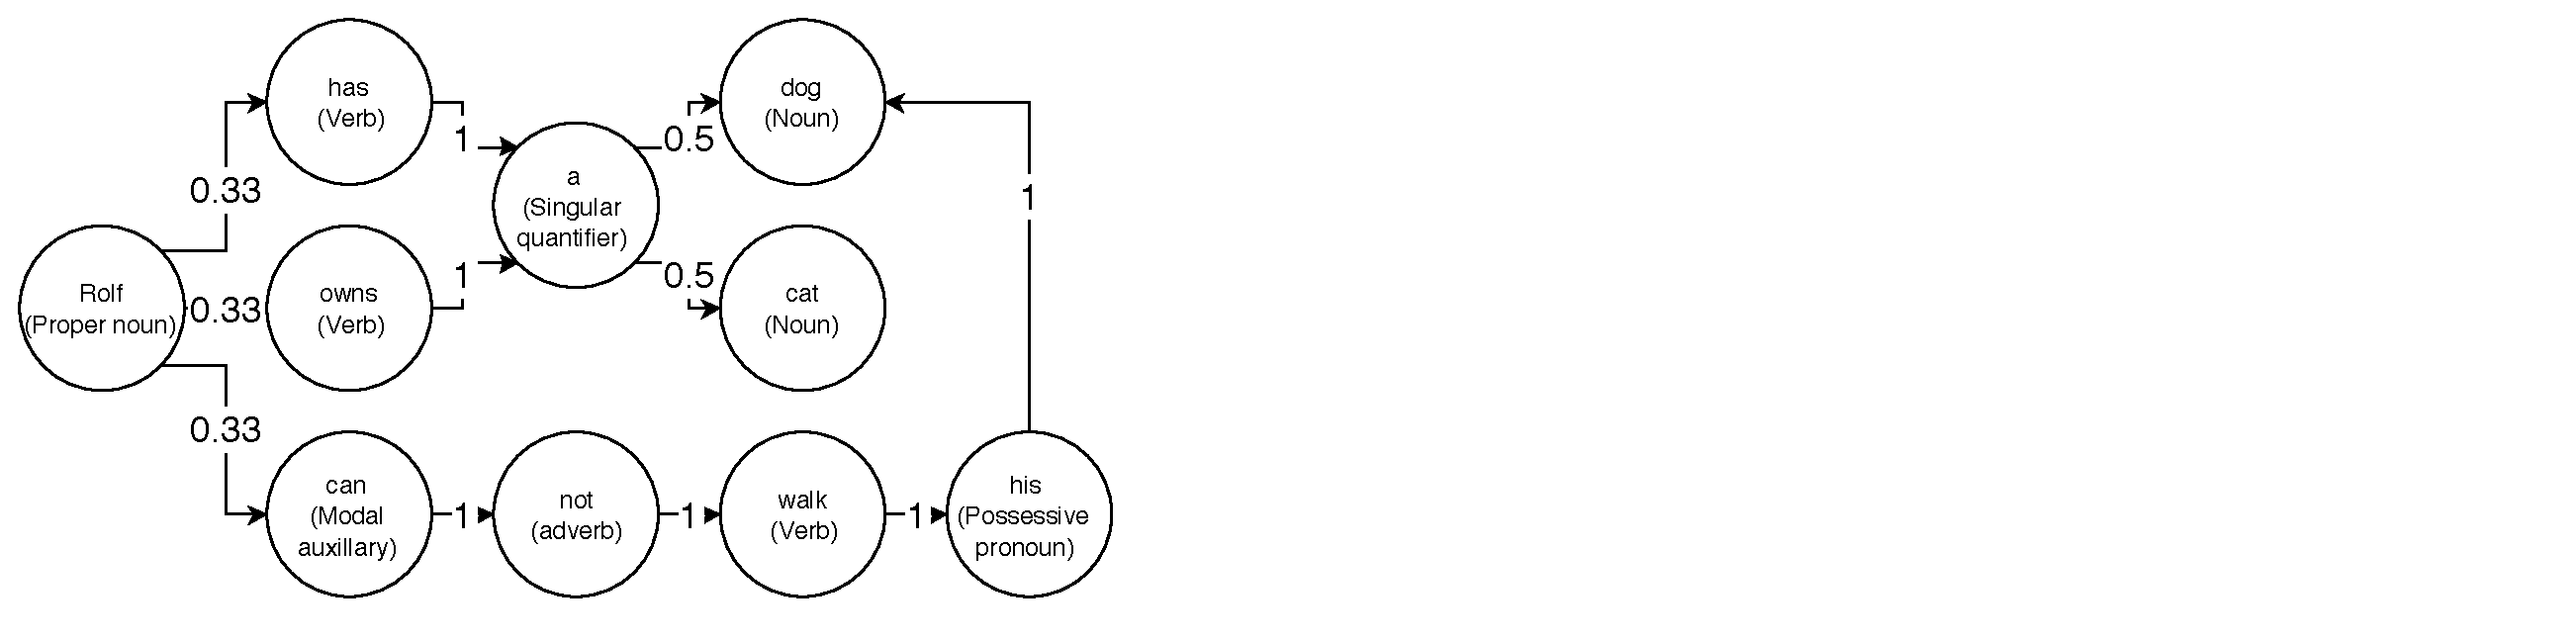
\includegraphics[width=0.49\linewidth]{Bigram1.pdf}}
  \hfill
  \subfigure[Bi-gram with constraints applied]{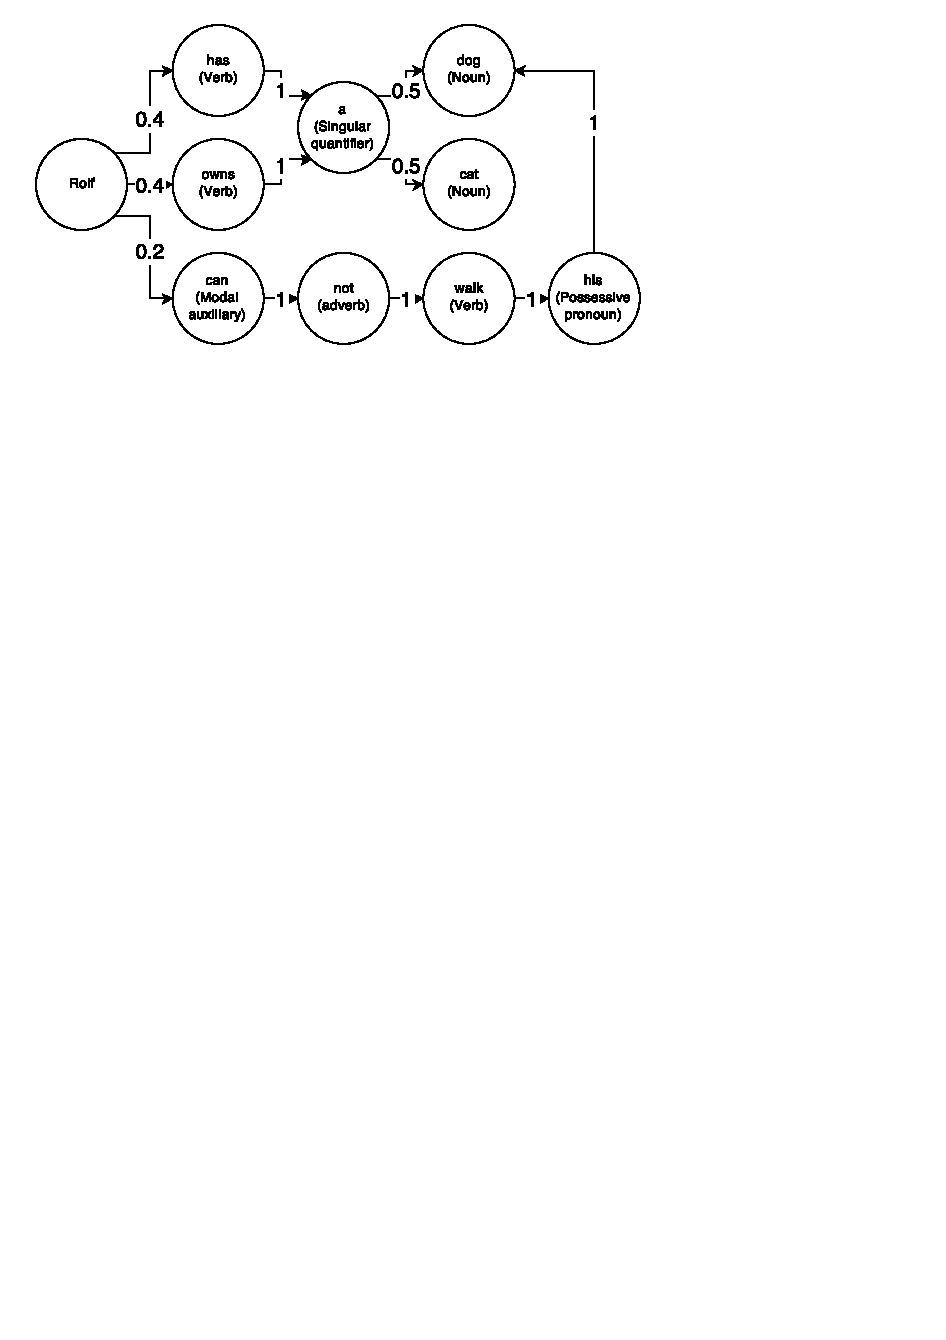
\includegraphics[width=0.49\linewidth]{Bigram2.pdf}}
  \hfill
  \caption{Bi-grams}
 \end{figure}



We can see in figure 1b that since both ''has`` and ''owns`` are verbs they are more probable to occur than ''can``, this is reflected in the new edges. 
This happens because the part-of-speech ''verb`` is more likely to follow a personal noun according to our transition matrix, and thus ''has`` and ''owns``, who are 
both verbs become even more likely to follow a personal noun. This method can then be further applied to a tri-gram, a four-gram or any n-grams that follows. 
Our experiments however will only use a bi-gram for the transition matrix, even if the Markov chain of words from the corpus is longer, 
the transitions are only observed with one previous state in consideration.

\subsubsection{Calculating uniqueness}
\label{subsec:calcuniq}
Since it is not possible to get a value on the semantic correctness of a sentence programatically we create a metric based on the uniqueness of a generated tweet based on how much of the tweet is copied straight from the corpus.
Because we use a tri-gram, three successive words will always be chosen from the corpus but anything more than that makes it less unique.

For example purposes we added these sentences to the limited corpus mentioned earlier:

\begin{tabular}{l}
``Mufasa is a dog with a purple tail.``\\
``Mufasa owns a yellow cat.``\\
``Jessica can not eat a yellow dog with a pink tail.``\\
``Steve has a shirt with a purple tail.``
\end{tabular}

% Räkna manuellt med limited corpus
\textbf{Example 1:} ``Rolf can not eat a yellow cat.``
	
It first matches "can not eat a yellow" since it is the largest continuous match. This match contains five words, which is two words longer than it has to be (since we use a tri-gram), this reduces uniqueness by 2. What is left is the strings "Rolf" and "cat", since each of these strings are shorter than three words the analysis stops here.

Thus this sentences uniqueness is $\frac{7 - 2}{7} \approx$ 71 percent.

\textbf{Example 2:} ``Rolf has a shirt with a yellow dog with a pink tail.``
	
The first match is "a yellow dog with a pink tail", reducing uniqueness by 4. Remaining is "Rolf has a shirt with" which matches "has a shirt with", further reducing uniqueness by 1. The analysis stops here since only "Rolf" is left.

Thus this sentence has a uniqueness of $\frac{12 - (4 + 1)}{12} \approx$ 58 percent.

\subsubsection{Corpus}
Initially discussed was the problem regarding the semantic correctness of a generalized tweet when it comes to generating tweets.
The average tweet is not semantically correct. This is not a problem in understandability for an experienced Twitter user,
but is a problem for the POS which can not recognize the words. Even if it could give it an ''unknown``-tag, predicting any kind of results would not be possible.

\begin{figure}[h!]
  \centering
  
\includegraphics[width=0.6\linewidth]{machine_learning}
  \caption{An example tweet}
\end{figure}

To solve this problem approximately one solution is to generate tweets for a specific user who mostly uses correct grammar and semantics when tweeting and tweets in English.
Carl Bildt, former foreign minister of Sweden, was chosen because of his active use of Twitter, 
that he tweets in English and that most of his tweets are in grammatically correct English.

\subsection{Implementation}
\label{sec:impl}
Data is collected in the form of tweets, by a target person, Carl Bildt, to be used as the corpus for the tweet generator. The data is filtered to remove unwanted elements such as hash-tags and web addresses.

The implementation relied on a Part-of-Speech tagger from Stanford's Natural Language Processing group. Each tweet is run through said tagger to get the lexical class of each word depending on context.
These lexical classes are then used as states for the transition matrix, more specifically they are used to see what lexical class usually follows any given lexical class, or terminates a sentence.

While iterating through the gathered data the preceding two words are stored as being words that are followed by the current word, including sentence terminating symbols such as '.' or '!'. This is then stored as a tri-gram.

When generating tweets two methods are used, first the tri-gram gets to select which words to use entirely on its own (Markov chain). Then the process is repeated but this time the tri-gram is constrained by which lexical class of words it is allowed to choose from, that class being whichever one the transition matrix has decided should follow (constrained Markov chain).

%%%%%%%%%%%%%%%%%%%%%%%%%%%%%%%%%%%%%%%%%%%%%%%%%%%%%%%%%%%%%
%%%%%%%%%%%%%%%%%%%%%%%%%%%%%%%%%%%%%%%%%%%%%%%%%%%%%%%%%%%%%
\section{Experimental results}
\label{sec:exps}

\subsection{Experimental setup}
10000 tweets with a length of between 30 and 140 characters was generated using both the Markov chain and the constrained Markov chain.
The maximum length of a tweet is 140 characters and 30 is an arbitrarily chosen lower bound.

Once generated the tweets are analysed for uniqueness by counting how many of the used words are from the same part of the corpus. However, since a tri-gram is used, three of the words have to appear in succession and thus are only counted if four or more of the words are from the same part of the corpus. This is then divided this by the number of words to get an average for the whole tweet, as described in section~\ref{subsec:calcuniq}.

\newpage
\subsection{Experiment}

\subsubsection{Uniqueness based on words in tweet}

\begin{figure}[h!]
  \hfill
  \begin{center}
  	{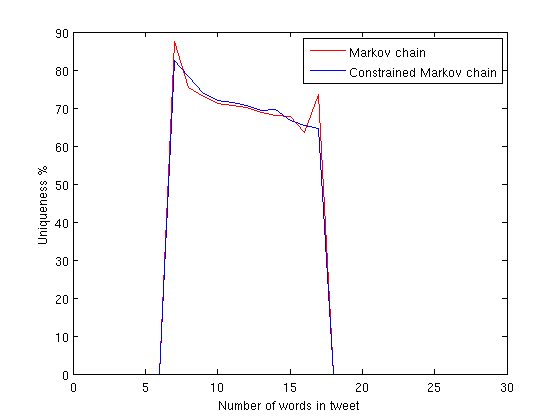
\includegraphics[width=300, height = 140]{UniqByNumWordsTweet.png}}
  \end{center}
  \caption{Uniqueness based on words in tweet}
 \end{figure}
 
 Uniqueness drops as the number of words in the tweet increases, both Markov chain and the constrained Markov chain decrease at  approximatively the same rate however. This is because of how the algorithm for uniqueness works, namely that if the tweet has 6 words then at worst it can take all 6 words from the same part of the corpus. This will result in a uniqueness of 50 percent, since this is a worst case scenario, it cannot be lower than this.
 
 \begin{figure}[h!]
   \hfill
   \begin{center}
  	{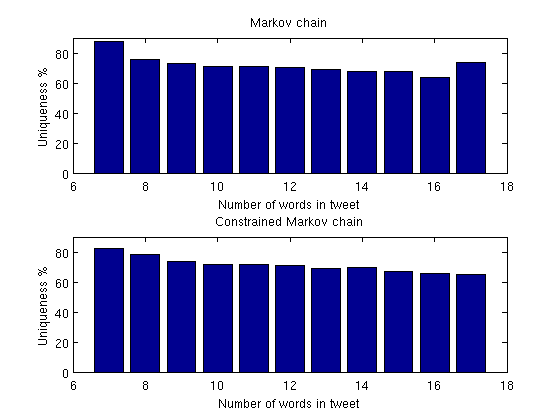
\includegraphics[width=280, height = 140]{UniqByNumWordsTweet2.png}}
  \end{center}
  \hfill
  \caption{Uniqueness based on words in tweet (Comparison)}
 \end{figure}
 
 On average the constrained Markov Chain produces tweets that are 71.04 percent unique and the Markov Chain has an average uniqueness of 70.29 percent. This means the constrained Markov chain constructs, on average, tweets that are 1.01 percent more unique.


\subsubsection{Number of tweets based on uniqueness}

\begin{figure}[h!]
  \hfill
  {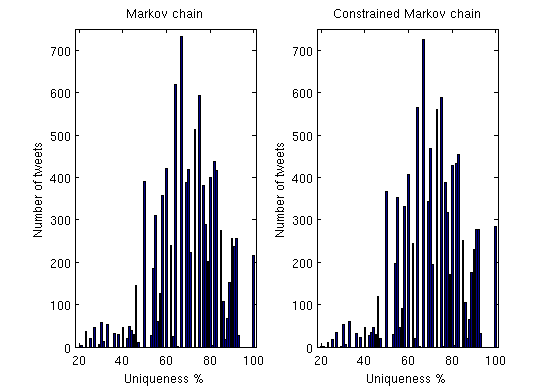
\includegraphics[width=1\linewidth, height = 165]{NumTweetsByUniq.png}}
  \caption{Number of tweets based on uniqueness}
 \end{figure}
 
 Here too, both the Markov chain and the constrained Markov chain have similar results as a whole but the Markov chain has more tweets with less uniqueness than the constrained Markov chain. The opposite is also true, the constrained Markov chain has more tweets with more uniqueness than the Markov chain.
 
  \begin{figure}[h!]
   \hfill
  {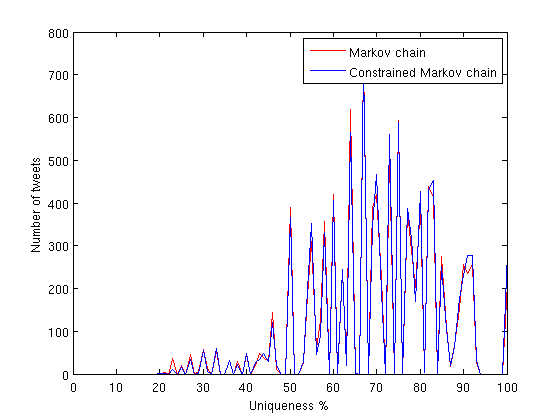
\includegraphics[width=1\linewidth, height = 165]{NumTweetsByUniq2.png}}
  \hfill
  \caption{Number of tweets based on uniqueness (Comparison)}
 \end{figure}

Figure 6 makes this more obvious, the graph shows that the Markov chain has visible spikes on the lower end of uniqueness (namely around 23 and 46 percent) and the constrained Markov chain has the same on the higher end (70, 82, 91 and 100 percent).

\subsubsection{Actual content of tweet}
Even though a way of mechanically analysing the semantic correctness of the tweets was not found, five generated example tweets analysed manually, for both methods.

\textbf{Markov chain}

% Punktlista
\begin{itemize}
\setlength\itemsep{-0.8em}
\item ``Of risk of situation in Ukraine. By Pyongyang standards.``
\item ``Victory Day has a great time!\hspace{0 cm}``
\item ``And clear messages from Brussels after two days. The final rally of the.``
\item ``Third capital today. Symbolic that US wins over Russia.``
\item ``Well, Cold War it was? For a day in the clowns''.``
\end{itemize}

\textbf{Constrained Markov chain}

% Punktlista
\begin{itemize}
\setlength\itemsep{-0.8em}
\item ``\selectlanguage{russian}Очевидно обострение экономической войны Russia is good.``
\item ``Truly alarming development in Bosnia.`` % INTE helt kopierad
\item ``Started the meeting in Brussels. Istanbul after a couple of grey suits as well.``
\item ``We have every reason to follow the different parts of Eastern Ukraine.``
\item ``PM's Reinfeldt of Sweden. Most of our world. Looks worse than a dog.``
\end{itemize}

Occasionally the beginning and end of the generated tweets are semantically incorrect, this is caused by the corpus filtering as the preceding and/or subsequent element has been removed from the corpus.

Languages are not filtered which means that sometimes there are strings of, for example, Russian that cannot be determined if the strings are semantically correct or not.

Otherwise the subjects of the generated tweets all seem to revolve around politics and foreign relations and could therefore possibly be from a foreign minister.

Based on generated tweets, it can seen that there is similarity of the semantic structure and content for both methods. 

\newpage
%%%%%%%%%%%%%%%%%%%%%%%%%%%%%%%%%%%%%%%%%%%%%%%%%%%%%%%%%%%%%
%%%%%%%%%%%%%%%%%%%%%%%%%%%%%%%%%%%%%%%%%%%%%%%%%%%%%%%%%%%%%
\section{Summary and Conclusions}
\label{sec:summary}
% Vad har vi kommit fram till?
The report compares generating natural language with a native tri-gram from a corpus with using a constrained Markov chain of order 2 to generate tweets seeming to originate from a specific person, which in the experiment was Carl Bildt. 
The tweets should thus be semantically correct and have a somewhat meaningful content.
In the results it can be seen that using a constrained Markov chain has a slight advantage over simply using a tri-gram in generating a diversity of content. 
However, there was seemingly no difference at all in the quality of the content. 
They did seem to be from Carl Bildt, since the topics of the tweets were affected by the words in his tweets. 
A lot of the generated tweets had a political theme where conflicts were discussed and political situations in different regions of the world. 


% Vad bidrog det med?
It was shown that applying constraints on a tri-gram made little difference rather than just using a tri-gram. The approach adds a lot of work for small gain, and that the gain results in mostly nonsensical text. When the diversity in the generated tweet increased so did the quality decrease.

% Hur kan våra resultat förbättras/förändras?
The constrained matrix only uses a bi-gram, if it would use a tri-gram for it's POS constraints, perhaps the outcome would have been different. The outcome would probably be affected by it, however it is hard to say whether it would improve the results a lot. If the Markov chain was constrained by another property than the sequence of POS in Carl's tweets the results could possibly be different. An alternative could be to generate a template with topics that divide the tweet into parts and let that be the constraint of the Markov chain instead.


%%%%%%%%%%%%%%%%%%%%%%%%%%%%%%%%%%%%%%%%%%%%%%%%%%%%%%%%%%%%%
%%%%%%%%%%%%%%%%%%%%%%%%%%%%%%%%%%%%%%%%%%%%%%%%%%%%%%%%%%%%%
\bibliographystyle{plainnat}
\newpage
\bibliography{reflist}


\end{document}